\chapter{Data Preprocessing}

There are different techniques used in learning in order to improve the accuracy of the model by preprocessing the data:

There are three common forms of data preprocessing a data matrix $X$, where we will assume that $X$ is of size $[N \times D]$ ($N$ is the number of data, $D$ is their dimensionality).

\begin{figure}[!htb]
  \centering
  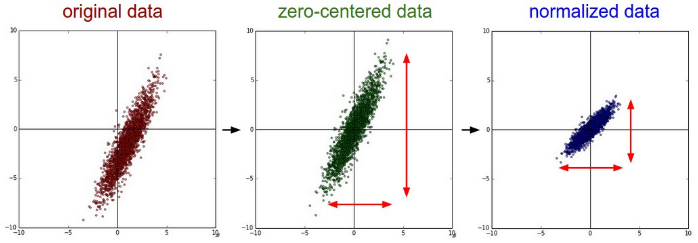
\includegraphics[width=0.7\textwidth]{Images/data_preprocessing/1.png}
  \caption{Preprocessing example 1}
\end{figure}

\begin{figure}[!htb]
  \centering
  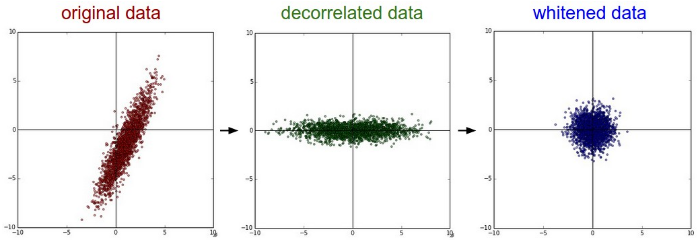
\includegraphics[width=0.7\textwidth]{Images/data_preprocessing/2.png}
  \caption{Preprocessing example 2}
\end{figure}

\paragraph*{Mean subtraction} Most common form of preprocessing. It involves subtracting the mean across every individual feature in the data, and has the geometric interpretation of centring the cloud of data around the origin along every dimension. In NumPy, this operation would be implemented as: \texttt{X -= np.mean(X, axis = 0)}. With images specifically, for convenience it can be common to subtract a single value from all pixels (e.g. \texttt{X -= np.mean(X)}), or to do so separately across the three color channels.

\paragraph*{Normalization} Refers to normalizing the data dimensions so that they are of approximately the same scale. There are two common ways of achieving this normalization. One is to divide each dimension by its standard deviation, once it has been zero-centered: (\texttt{X /= np.std(X, axis = 0)}). Another form of this preprocessing normalizes each dimension so that the min and max along the dimension is -1 and 1 respectively. It only makes sense to apply this preprocessing if you have a reason to believe that different input features have different scales (or units), but they should be of approximately equal importance to the learning algorithm. In case of images, the relative scales of pixels are already approximately equal (and in range from 0 to 255), so it is not strictly necessary to perform this additional preprocessing step.

\paragraph*{PCA} The reason why one would want to use PCA is if one expects that many of the features are in fact dependent. This would be particularly handy for Naive Bayes where independence is assumed. Most datasets are far too large to use PCA. Attention: PCA complexity is $~O(n^3)$, so more sophisticated methods are required. But if your dataset is small, and you don't have the time to investigate more sophisticated methods, then by all means go ahead and apply an out-of-box PCA for feature selection.

\paragraph*{Whitening} Takes the data in the eigenbasis and divides every dimension by the eigenvalue to normalize the scale. The geometric interpretation of this transformation is that if the input data is a multi-variable Gaussian, then the whitened data will be a Gaussian with zero mean and identity covariance matrix.

\subsection*{Deep Learning with images}
For Deep Learning for images we will only use: center our data to zero. To do so, for each pixel, compute its mean across all the dataset and subtract the resulting mean image to all the training samples. If you have more than one channel (e.g. RGB) do it for each of the channels separately.
